\chapter{Αποτελέσματα Προσομοιώσεων}
Το παρόν κεφάλαιο έχει ως στόχο την εξαγωγή αποτελεσμάτων της επίδοσης του
ελεγκτή. Οι προσομοιώσεις του δυναμικού συστήματος πραγματοποιείται μέσω κώδικα 
που έχει συντεθεί στην προγραμματιστική γλώσσα \tl{MATLAB}.

Η στάθμιση των ιδιοτιμών του συστήματος έχει πραγματοποιηθεί στην αντίστοιχη 
ενότητα στο προηγούμενο κεφάλαιο. Τα αντίστοιχα αποτελέσματα του ονομαστικού 
ελεγκτή για ακολουθία τροχιών αναφοράς και με επιβολή διαταραχών παρουσιάζονται 
στην προαναφερθείσα ενότητα. Για τις διάφορες περιπτώσεις που προσομοιώθηκαν, θα
εξεταστεί η επίδοση του συνολικού ελεγκτή.

Αρχικά, η αξιολόγηση της δυνατότητας εξασθένισης διαταραχών από τον ελεγκτή 
γίνεται βάσει της παραμέτρου $\gamma$. Μειώνοντας την τιμή της συγκεκριμένης 
παραμέτρου, αναμένουμε μείωση της επιρροής των διαταραχών στην έξοδο του 
συστήματος. Σε σύγκριση με τις βηματικές μεταβολές που επιβλήθηκαν στον 
ονομαστικό ελεγκτή, παρουσιάζονται οι αποκρίσεις των μεταβλητών εξόδου για 
διαφορετικές τιμές της παραμέτρου $\gamma$.

\begin{figure}[htb!]
    \centering
    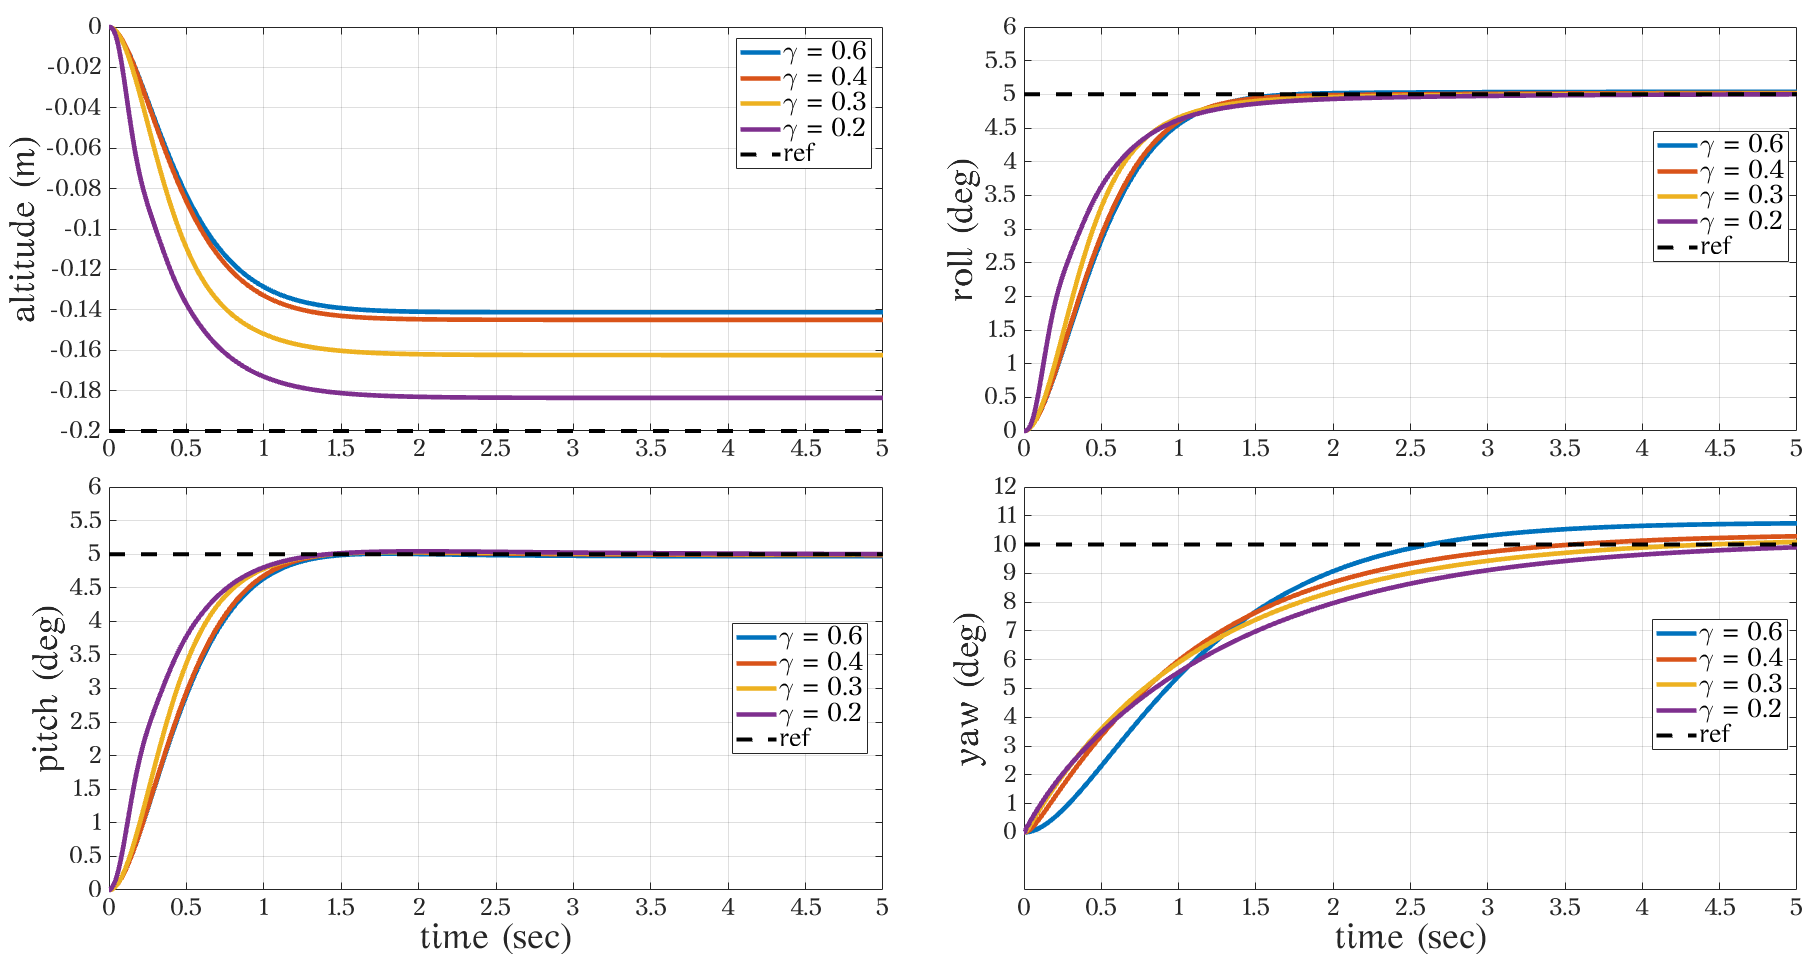
\includegraphics[width=1\textwidth]{Results/step_resp_gamma.png}
    \caption{Βηματικές Μεταβολές Μεταβλητών Εξόδου}
    \label{fig:step_d}
\end{figure}
Από το σχήμα (\ref{fig:step_d}), επιβεβαιώνεται η θεώρηση ότι με μείωση της 
παραμέτρου $\gamma$, το μόνιμο σφάλμα μειώνεται. Επιπλέον με αύξηση της $\gamma$
πάνω από μία τιμή δεν παρατηρείται σημαντική διαφορά στην επίδοση του ελεγκτή, 
εφόσον η συνεισφορά του αρχικού ελεγκτή γίνεται ισχυρότερη.

Η σύγκριση των τιμών $\gamma$ πρέπει να πραγματωθεί και για ακολουθία τροχιών
αναφοράς. Απαιτείται από τον ελεγκτή να πετύχει ημιτονοειδείς τροχιές αναφοράς 
στις γωνίες $\theta$ και $\psi$.
\begin{figure}[htb!]
    \centering
    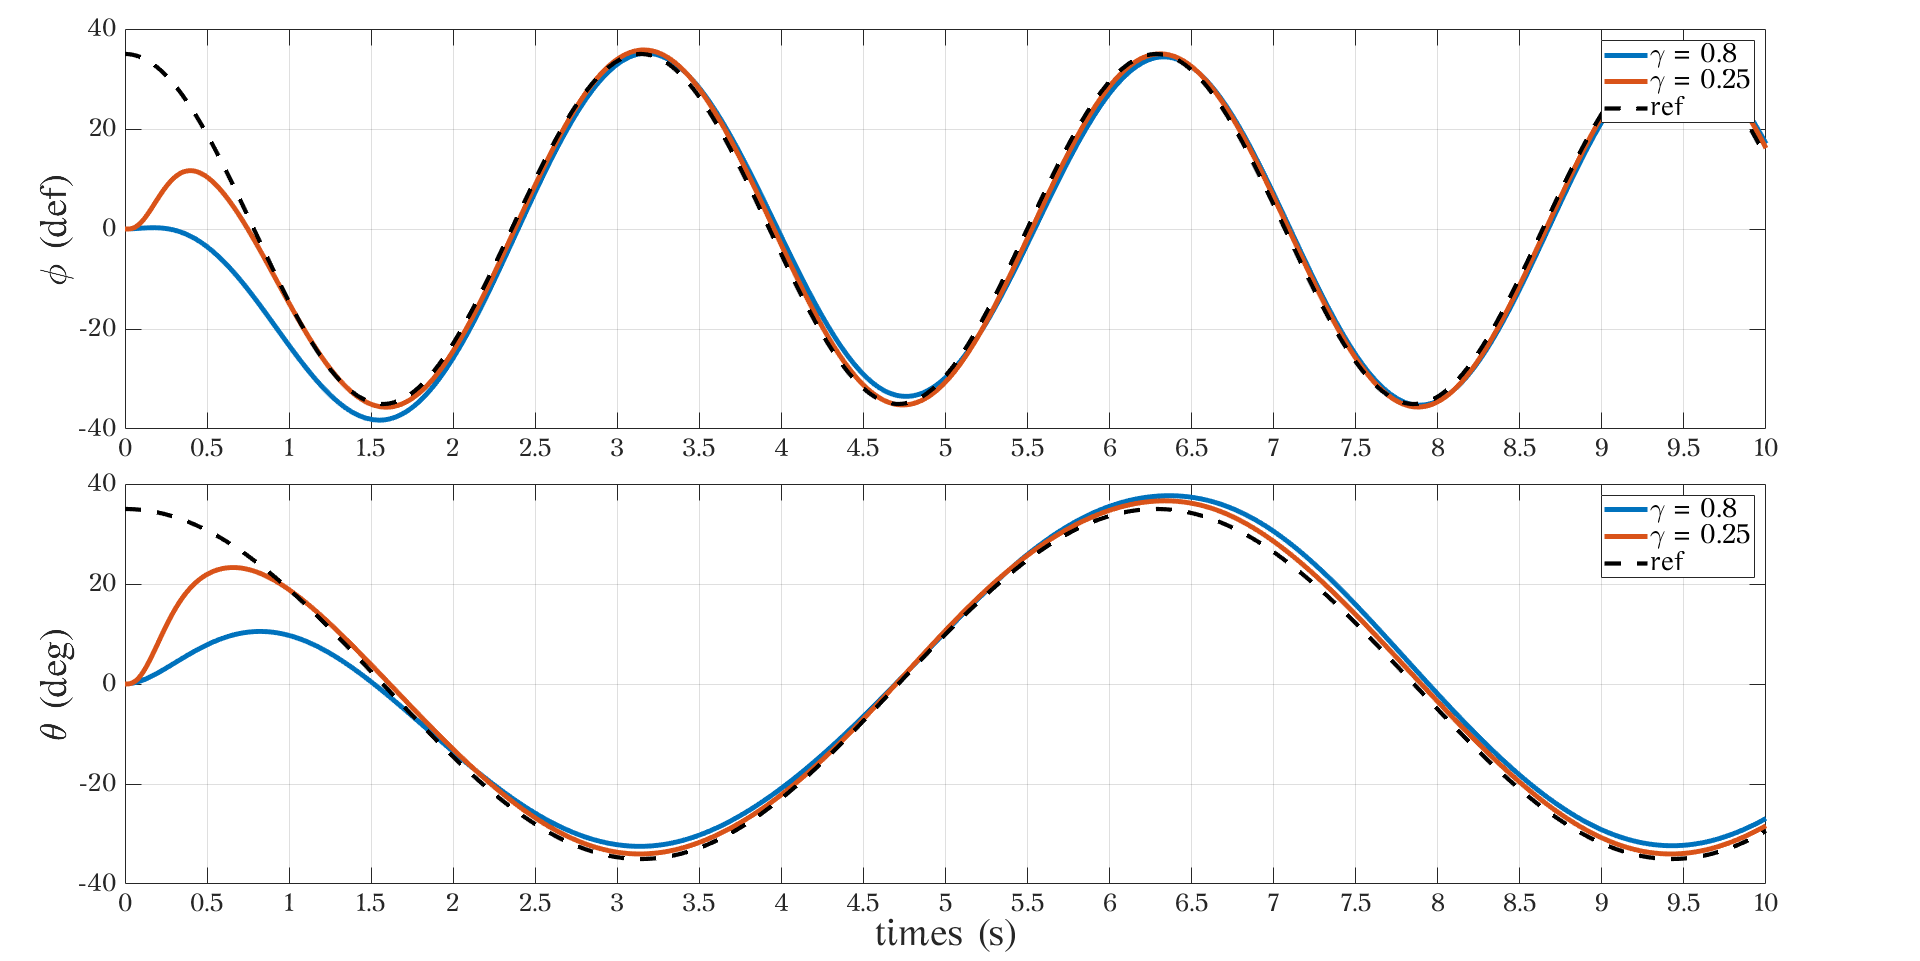
\includegraphics[width=1\textwidth]{Results/phi_theta.png}
    \caption{Ακολούθηση σήματος αναφοράς γωνιών $\theta$ και $\psi$.}
    \label{fig:roll_pitch_res}
\end{figure}
Όπως φαίνεται στο σχήμα (\ref{fig:roll_pitch_res}) και στις δύο περιπτώσεις η 
απόκριση βελτιώνεται αισθητά με τη μείωση της $\gamma$. Αρχικά και στις δύο 
περιπτώσεις η απόκλιση από την επιθυμητή τιμή είναι μικρότερη όταν $\gamma$ 
μικρότερο. Ένα συμπέρασμα, που προκύπτει εδώ σε σχέση με την ακολούθηση σταθερών
σημάτων, είναι πως η μείωση της παραμέτρου $\gamma$ κάνει την επίδοση 
γρηγορότερη, όπως παρατηρείται στα πρώτα δευτερόλεπτα τις συγκεκριμένης 
προσομοίωσης. 

Τέλος, γίνεται σύγκριση της περίπτωσης απογείωσης του τρικοπτέρου και ανύψωση 
του μέχρι τα $20 m$ και έπειτα την περιστροφή του γύρω από τον $z$ άξονα του 
αεροχήματος για την επίτευξη του ζητούμενου προσανατολισμού. Στην πρώτη 
περίπτωση (σχήματα \ref{fig:takeoff_wo_1}, \ref{fig:takeoff_wo_2}) παρατηρούμε 
τον ονομαστικό ελεγκτή να αντιδράει σε μόνιμες διαταραχές και διαταραχές που 
προκύπτουν από την σχετική ταχύτητα του ανέμου με την έλικα. Στην δεύτερη 
περίπτωση (σχήματα \ref{fig:takeoff_w_1}, \ref{fig:takeoff_w_2}), ο ελεγκτής 
λειτουργεί με εξασθένιση διαταραχών, με επιλεγμένη παράμετρο $\gamma = 0.3$.
\begin{figure}[H]
    \centering
    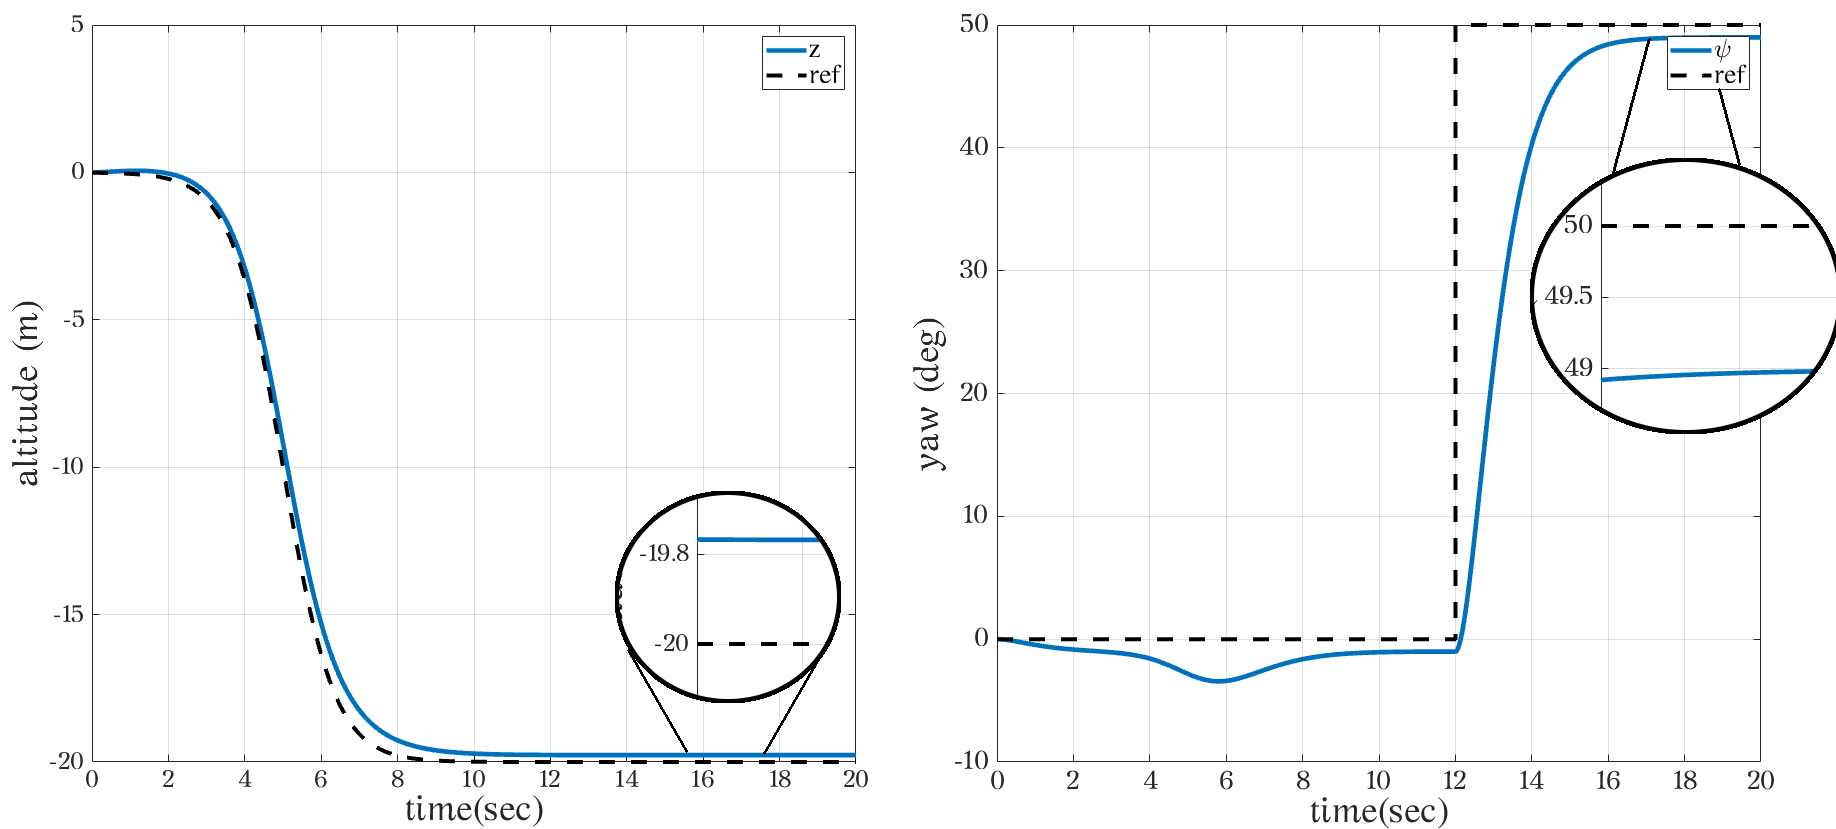
\includegraphics[width=0.85\textwidth]{Results/sigmoid_wo_1.png}
    \caption{Ύψος και προσανατολισμός χωρίς εξασθένιση διαταραχών για αιώρηση.}
    \label{fig:takeoff_wo_1}
\end{figure}
\begin{figure}[H]
    \centering
    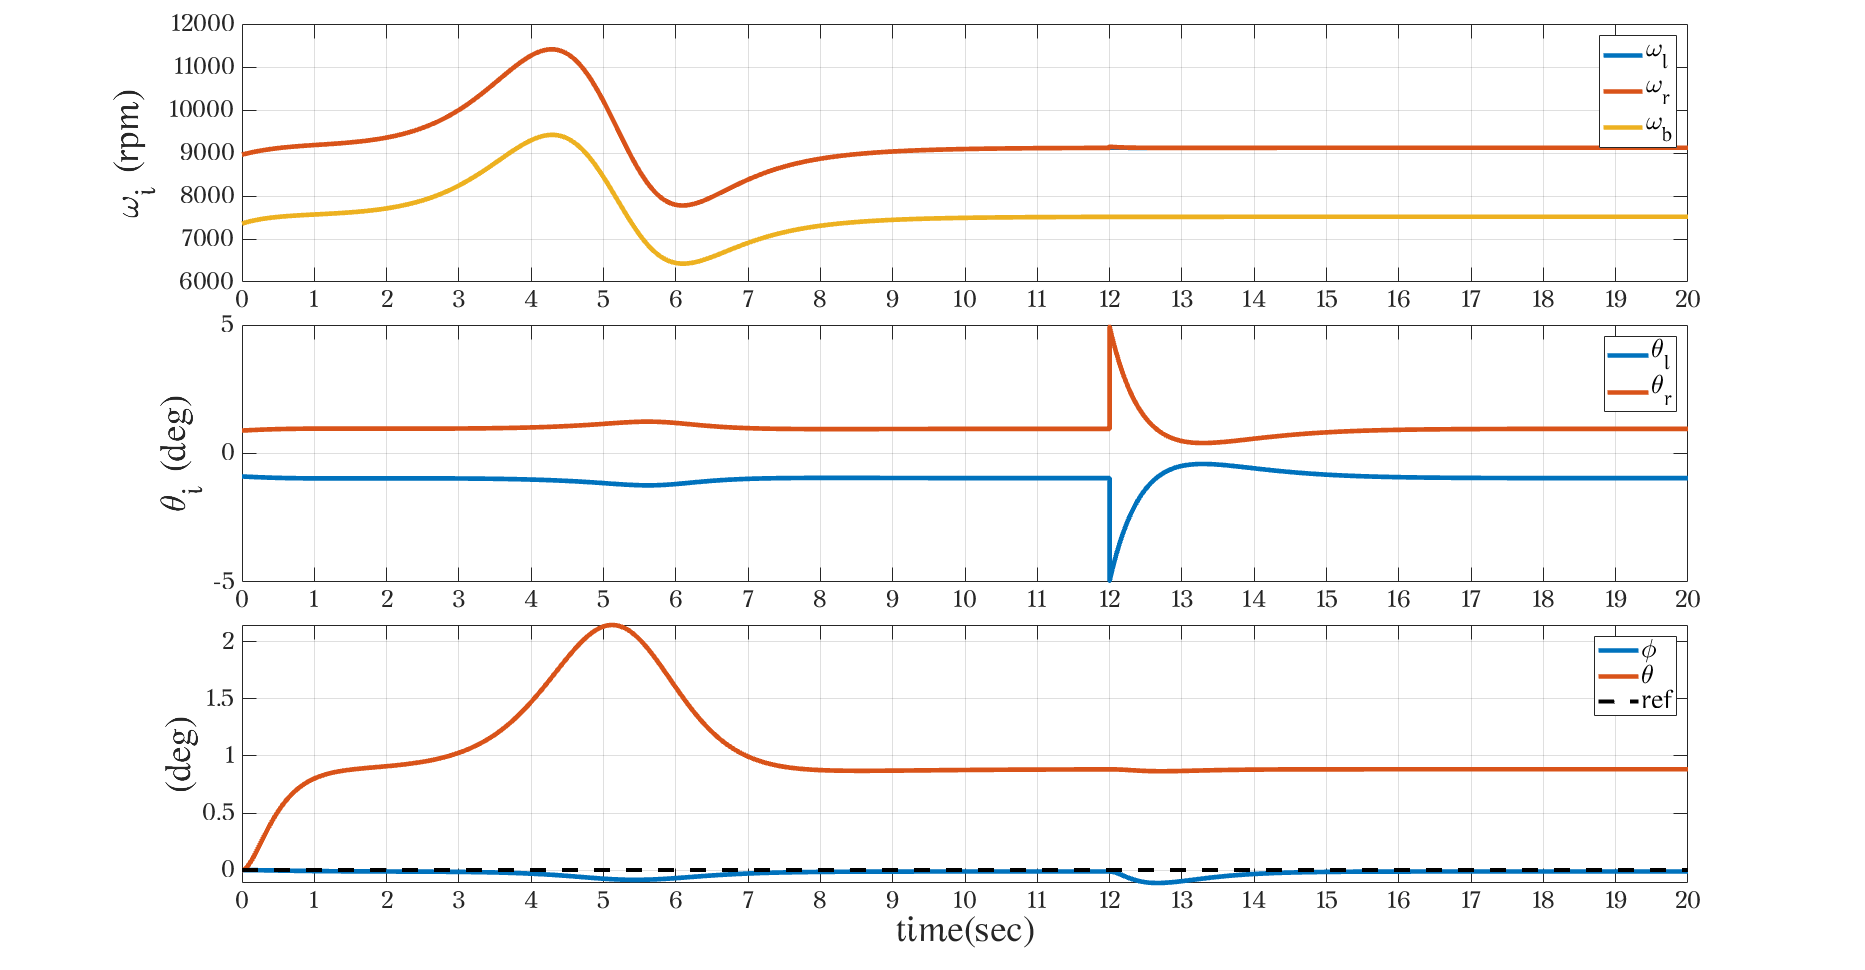
\includegraphics[width=0.85\textwidth]{Results/sigmoid_wo_2.png}
    \caption{Ενεργοποιητές, γωνίες \tl{euler} χωρίς εξασθένιση διαταραχών για 
    αιώρηση.}
    \label{fig:takeoff_wo_2}
\end{figure}
\begin{figure}[H]
    \centering
    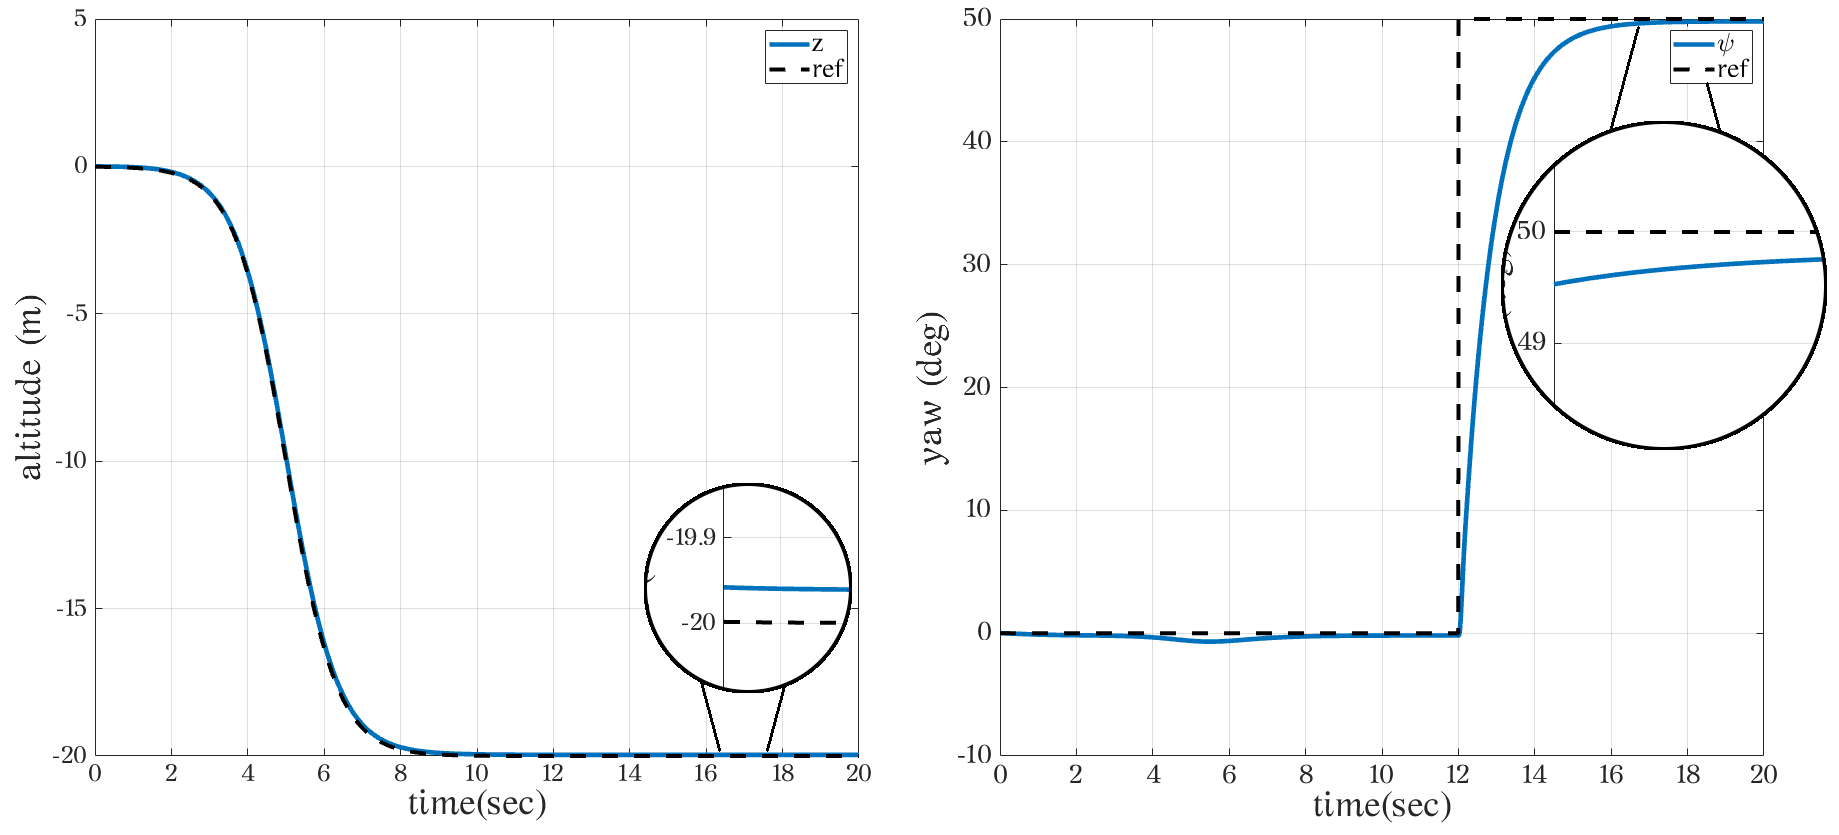
\includegraphics[width=0.85\textwidth]{Results/sigmoid_w_1.png}
    \caption{Ύψος και προσανατολισμός με εξασθένιση διαταραχών για αιώρηση.}
    \label{fig:takeoff_w_1}
\end{figure}
\begin{figure}[H]
    \centering
    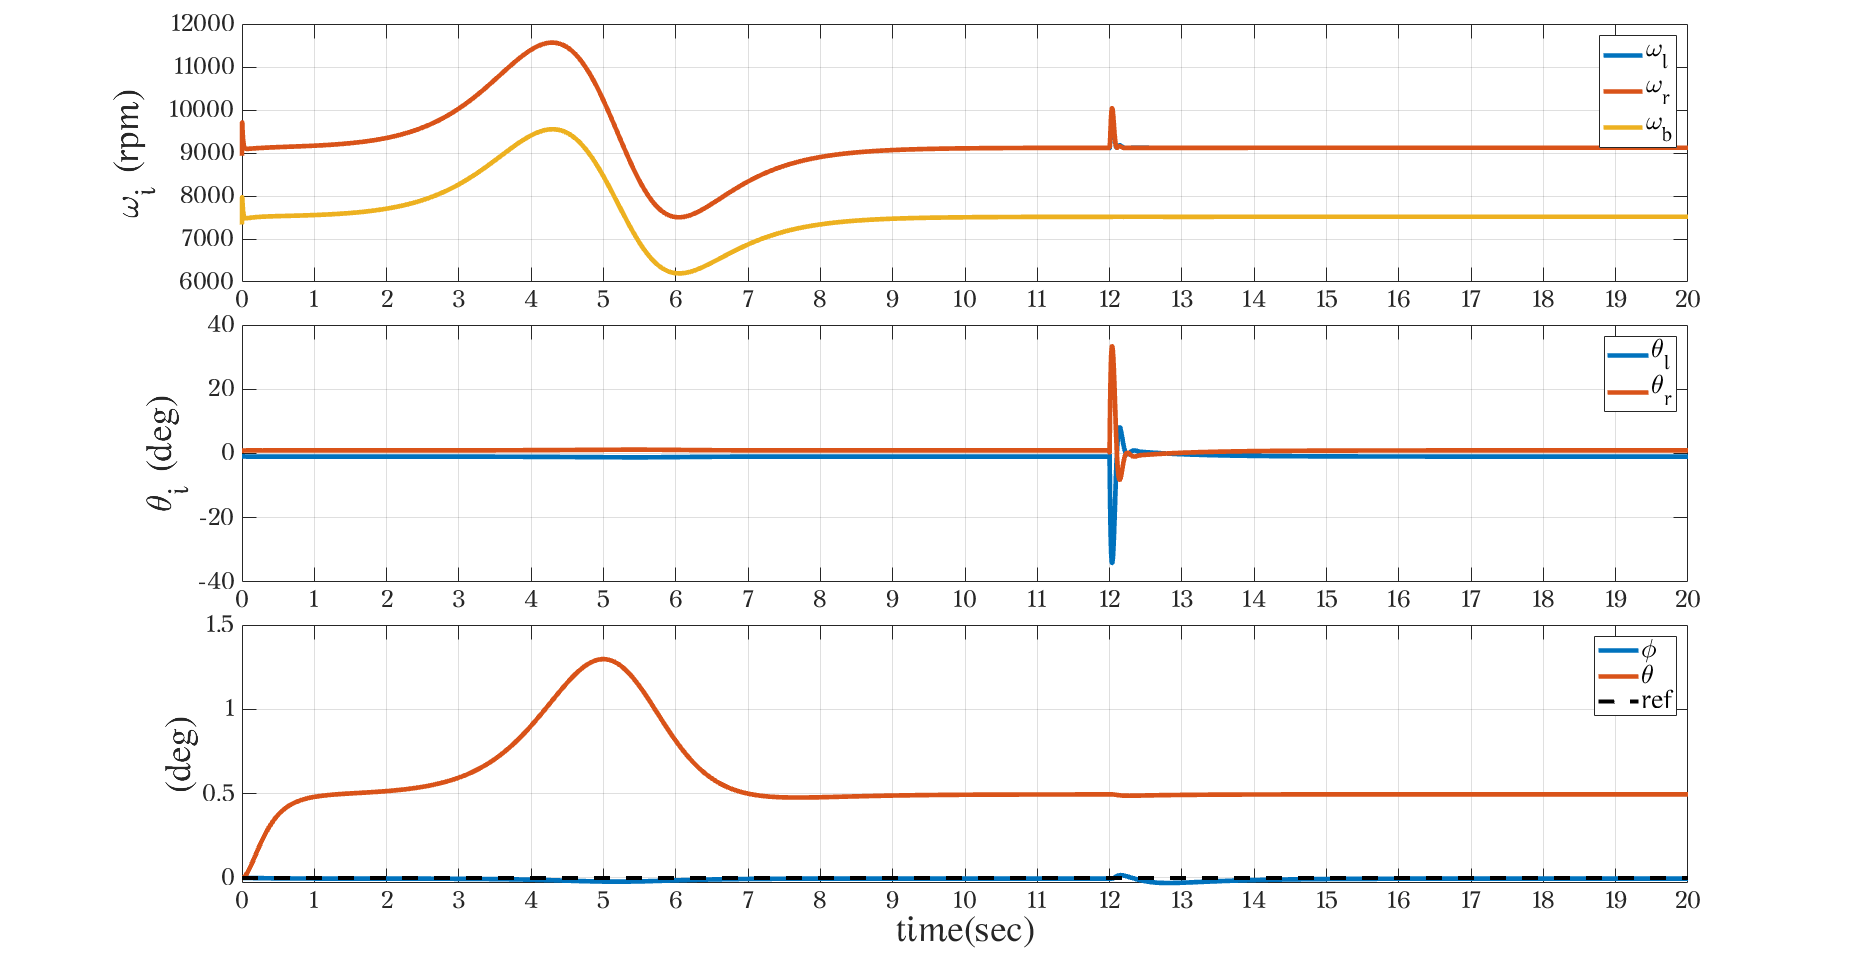
\includegraphics[width=0.85\textwidth]{Results/sigmoid_w_2.png}
    \caption{Ενεργοποιητές, γωνίες \tl{euler} με εξασθένιση διαταραχών για 
    αιώρηση.}
    \label{fig:takeoff_w_2}
\end{figure}

Απο τα παραπάνω διαγράμματα, παρατηρείται στις μεταβλητές εξόδου μείωση άνω του
$50\%$ των μόνιμων αποκλίσεων. Επιπλέον, ενώ στον ονομαστικό ελεγκτή 
παρατηρούνται μικρές γωνίες δράσης των σερβομηχανισμών αλλά για μεγάλο χρονικό 
διάστημα. Για τον συνολικό ελεγκτή οι αντίστοιχες γωνίες είναι μεγαλύτερες 
αλλά ακαριαίες. Αυτό συμβαίνει διότι ως στόχος του ελεγκτή είναι η απόσβεση της 
δράσης των διαταραχών, χωρίς την βέλτιστη ενεργειακά λύση για τις δράσεις. 

Στη συνέχεια  παρουσιάζεται η δράση της εξασθένισης διαταραχών για το σενάριο 
του σχήματος \ref{fig:dist_1}. Στόχος εδώ είναι να περιορισθεί η απόκλιση που 
προκαλείται παραπλεύρως στο ύψος \tl{z} καθώς και των γωνιών \tl{euler}, μιάς 
και η διαταραχή που προκαλείται από τον σχετικό άνεμο στις προπέλες αποτελεί 
σημαντική μη σταθερή διαταραχή που αλλοιώνει αρκετά την επίδοση. Στην πρώτη 
περίπτωση εφαρμόζεται ελεγκτής με $\gamma = 0.8$ και τα αποτελέσματα φαίνονται 
στο \ref{fig:dist_80}.
\begin{figure}[H]
    \centering
    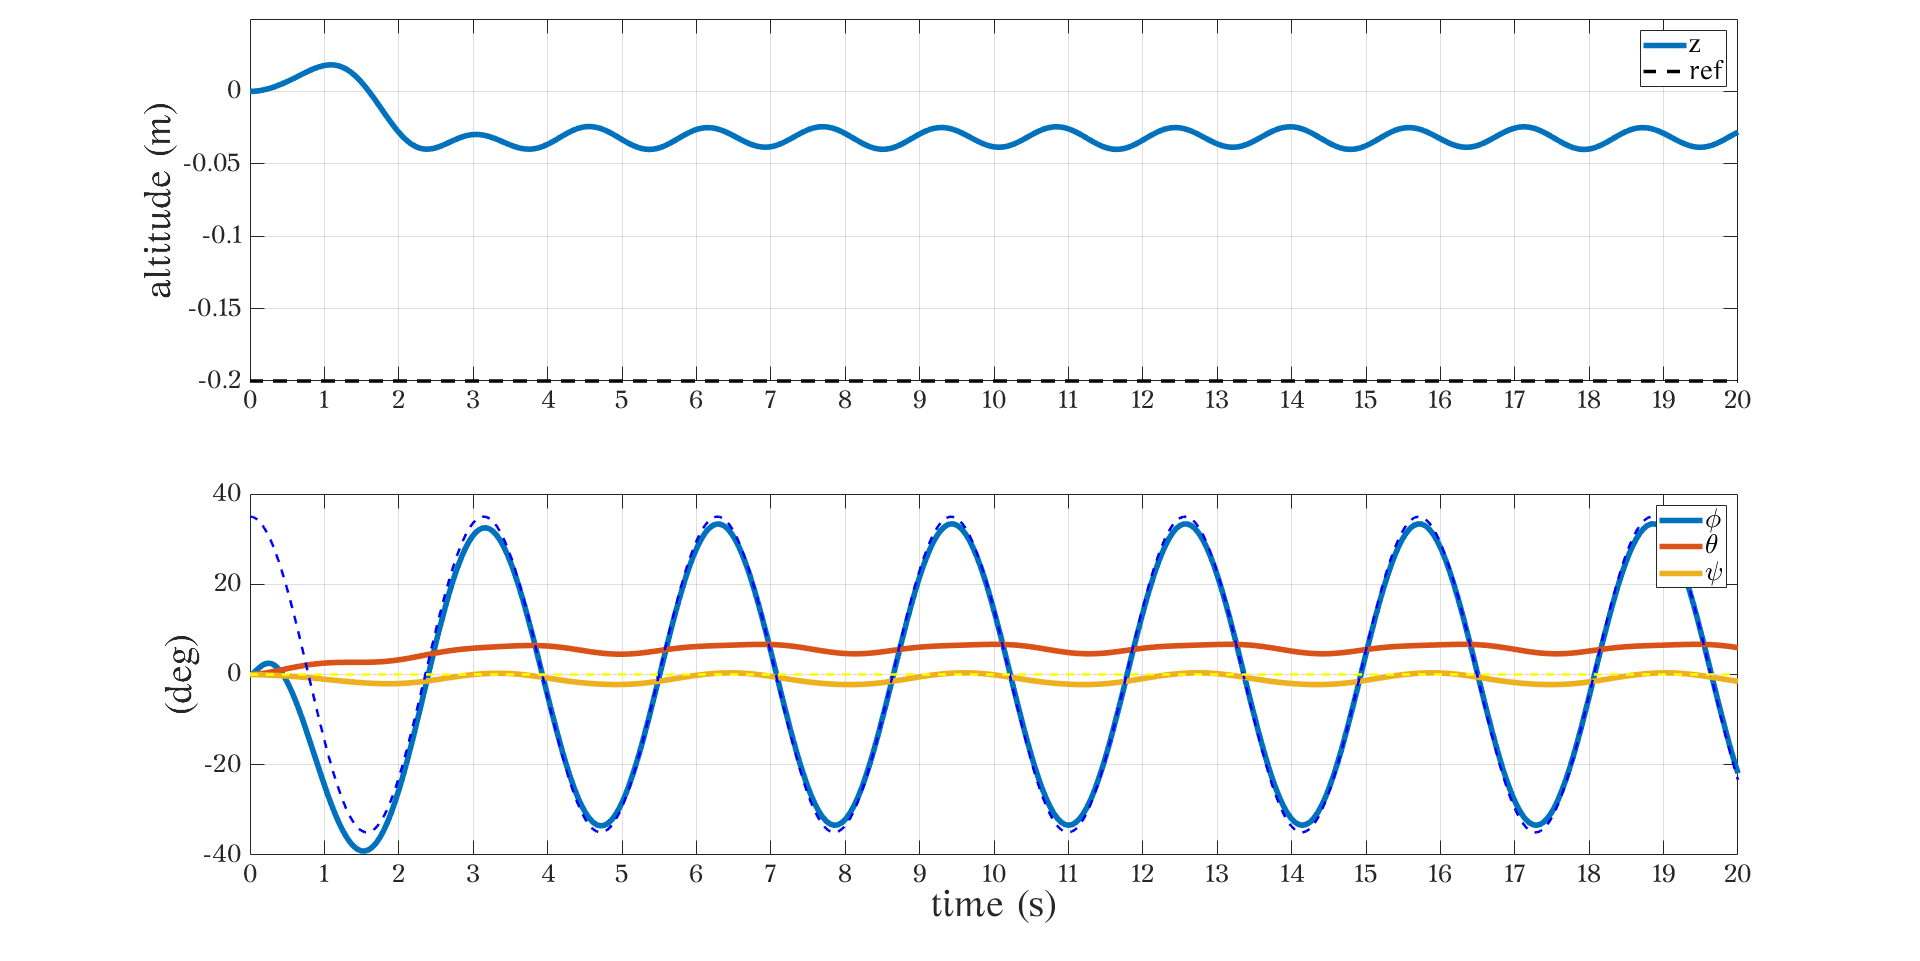
\includegraphics[width=0.85\textwidth]{Results/dist_gamma_80.png}
    \caption{$\gamma$ = 0.8.}
    \label{fig:dist_80}
\end{figure}
Στην πρώτη περίπτωση εφαρμόζεται ελεγκτής με $\gamma = 0.3$ και τα αποτελέσματα 
φαίνονται στο σχήμα \ref{fig:dist_30}.
\begin{figure}[H]
    \centering
    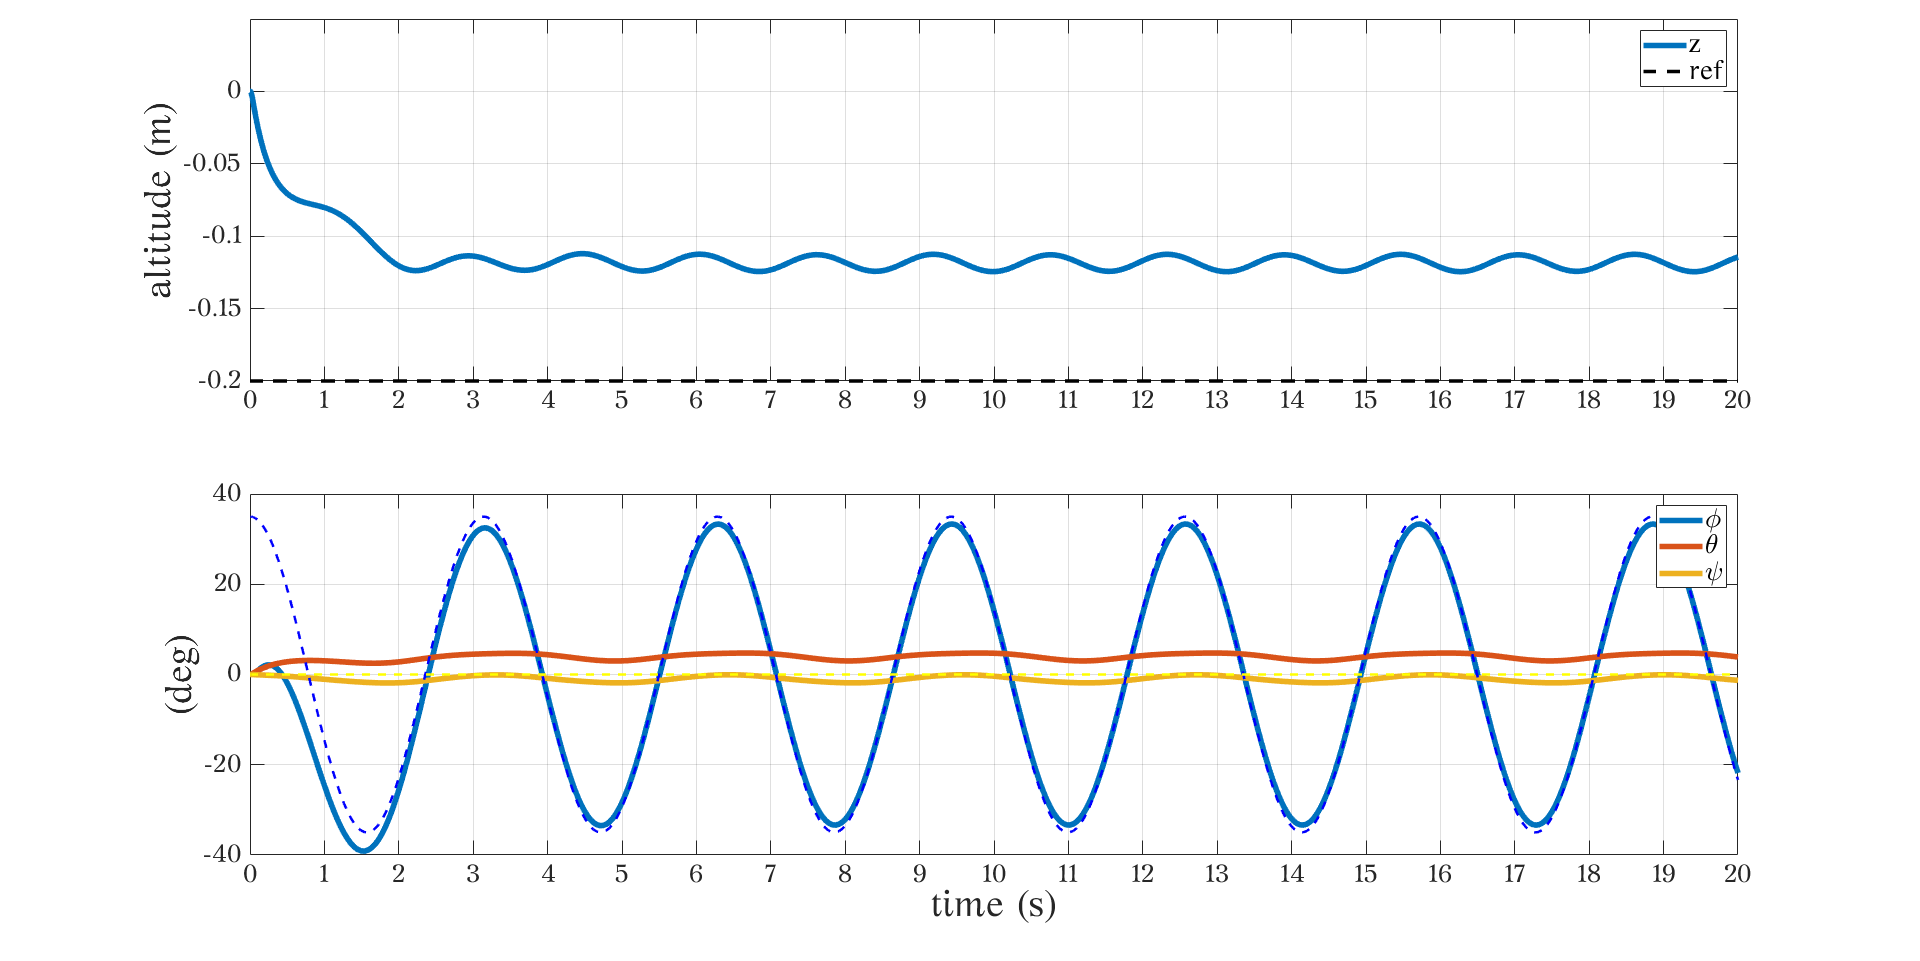
\includegraphics[width=0.85\textwidth]{Results/dist_gamma_30.png}
    \caption{$\gamma$ = 0.3.}
    \label{fig:dist_30}
\end{figure}
Όπως παρατηρεί κανείς, οι αποκλίσεις από την επιθυμητή τιμή μειώνονται αναλόγως 
την τιμή της παραμέτρου $\gamma$. Με αυτό το σενάριο, μπορεί να αντιληφθεί 
κανείς ότι ο ελεγκτής δρα κατά των δυναμικών διαταραχών αποτελεσματικά. Αξίζει 
να σημειωθεί πως το σενάριο που ασχολούμαστε αποτελεί ακραία συνθήκη 
λειτουργίας, κι έτσι η απόκλιση του ύψους είναι αποδεκτή. Σε πιό ομαλές 
συνθήκες, η απόκλιση του \tl{z} θα είναι χαμηλότερη από την τάξη μεγέθους των 
$10 cm$, η οποία αποτελεί ικανοποιητική απόκλιση για τις απαιτήσεις του 
συστήματος.

Από τις προσομοιώσεις καθώς και από την σύνθεση του ελεγκτή, είναι φανερό ότι η
παραμετροποίηση του κατασκευασμένου ελεγκτή γίνεται μόνο με τον ορισμό 
επιθυμητών ιδιοτιμών των πινάκων $K_1, \, K_2$ και την επιλογή επιθυμητής μείωσης 
διαταραχών $\gamma$. Έτσι, επιτυγχάνονται ικανοποιητικές αποκρίσεις χωρίς την 
σύγχυση που προκαλείται απο την ύπαρξη πολλών παραμέτρων. 